\chapter{Evaluation}\label{chap:evaluation}
\ifpdf
    \graphicspath{{Evaluation/Figs/Raster/}{Evaluation/Figs/PDF/}{Evaluation/Figs/}}
\else
    \graphicspath{{Evaluation/Figs/Vector/}{Evaluation/Figs/}}
\fi

To evaluate the performance of FAT-Pointer based range addresses a sample implementation we used
the morello board with CheriBSD's Benchmark ABI\cite{noauthor_benchmark_nodate} compilation mode for accurate performance recordings. 
The evaluation is to identify CheriBSD's default memory allocator SnMalloc against the prototype memory 
allocator using the contribution of this paper in terms of: 
To assess the performance of FAT-Pointer-based range addressing in the sample implementation, we utilized the 
Morello board running CheriBSD in Benchmark ABI compilation mode to ensure precise performance measurements. 
The evaluation focuses on comparing CheriBSD's default memory allocator, SnMalloc, against the prototype 
memory allocator developed in this study, with particular attention to the following aspects:

\begin{table}[!ht]
  \centering
  \begin{tabular}{|l|l|l|l|l|}
  \hline
      Metric name & type of graph & tool used & x axis & y axis \\ \hline
      DTLB L1 read & line graph & Pmcstat & Time & DTLB L1 reads (each second) \\ \hline
      DTLB L2 read & line graph & Pmcstat & Time & DTLB L2 reads (each second) \\ \hline
      DTLB walk & line graph & Pmcstat & Time & DTLB Walks (each second) \\ \hline
      L1 cache miss & line graph & Pmcstat & Time & L1 cache miss (each second) \\ \hline
      Wall clock run time & bar graph & time & Benchmarks & Time \\ \hline
  \end{tabular}
\end{table}

\subsection{Benchmarks used}:
To conduct the evaluations, we utilized the COZ\cite{curtsinger_coz_2015} benchmark suite, a well-regarded tool specifically designed 
to measure and analyze performance improvements in concurrent programs. The COZ benchmark suite provides a
robust framework for identifying bottlenecks and evaluating the performance impact of various optimization
techniques. By leveraging COZ, developers can gain precise insights into the efficiency and scalability of
their concurrent code, making it an ideal choice for rigorous performance analysis.

From the extensive set of benchmarks provided by COZ, we selected four representative C programs. 
These programs were chosen based on their relevance to common concurrent programming patterns and
their ability to effectively demonstrate the strengths and weaknesses of different optimization 
strategies. The selected programs cover a range of concurrency scenarios, ensuring a comprehensive
evaluation of performance improvements.

By implementing these modifications, we ensured that the selected C programs not only adhered to
CHERI's security model but also maintained their functional and performance characteristics. 
This allowed us to effectively use the COZ benchmark suite to analyze the performance in a CHERI-enhanced environment.

\begin{figure}[h]
  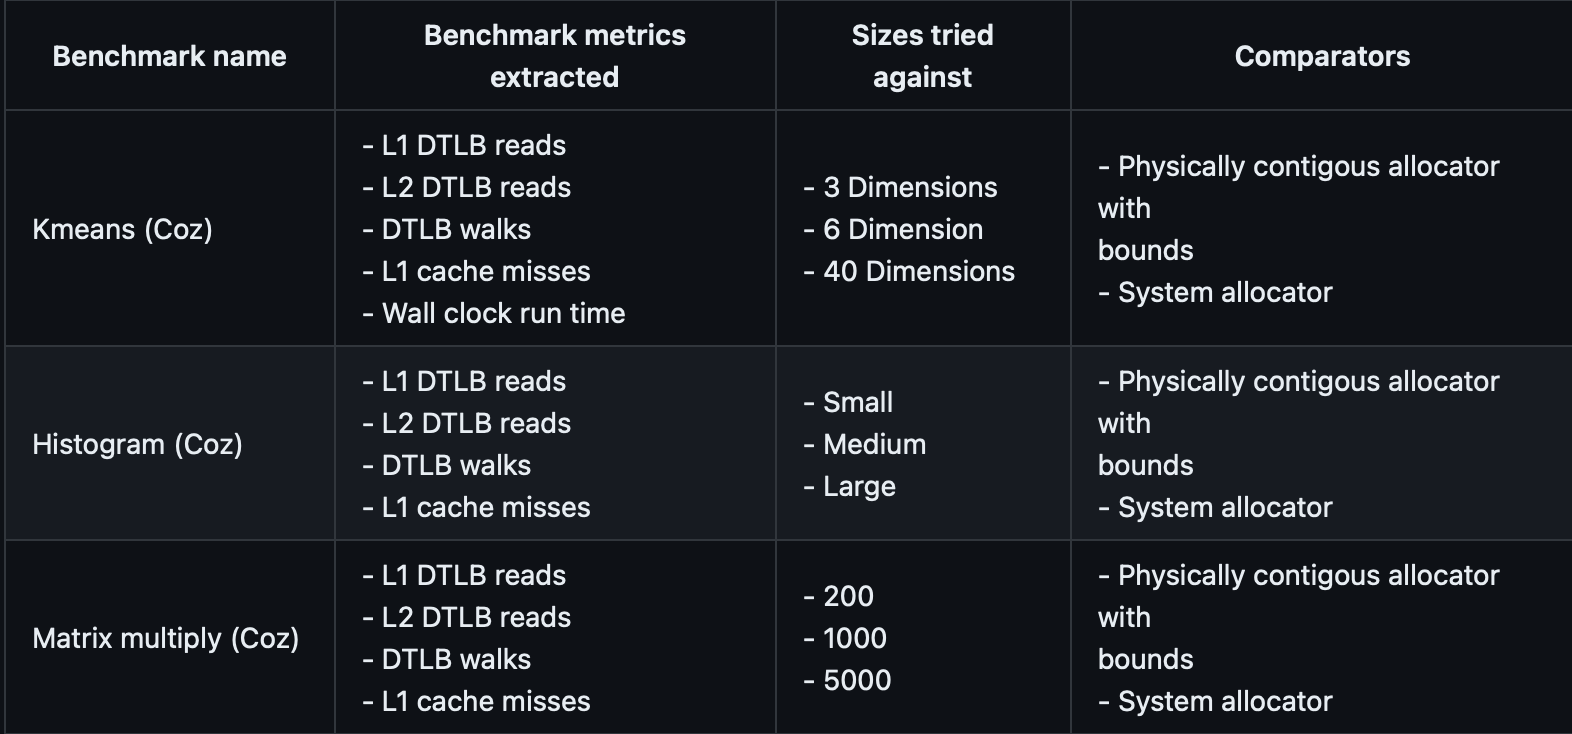
\includegraphics[width=0.8\textwidth]{diagrams/expirement-runs.png}
\end{figure}

\subsection{DTLB L1 reads:}
The Graphs above represent the DTLB L1 reads which is a Performance counter from the ARM specs. 
The counter increments for every Memory-read or Memory-write operation that necessitates an 
access to the Level 1 data or unified Translation Lookaside Buffer (TLB). 
Each access to a TLB entry is counted including multiple accesses caused by single instructions.


% L1 TLB graphs
\begin{figure}
  \begin{subfigure}{\linewidth}
  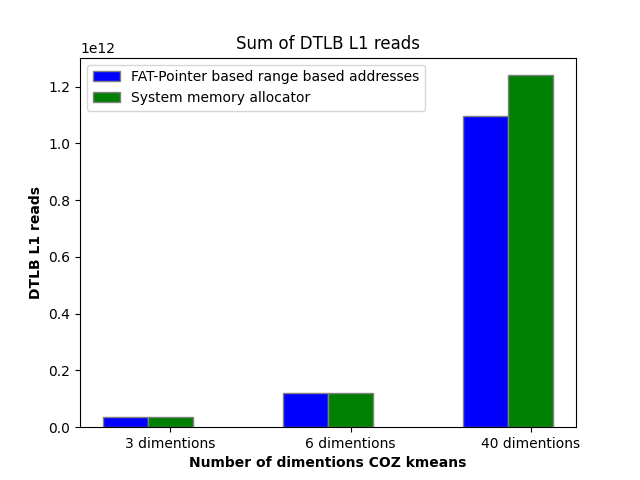
\includegraphics[width=.5\linewidth]{l1-tlb-kmeans.png}\hfill
  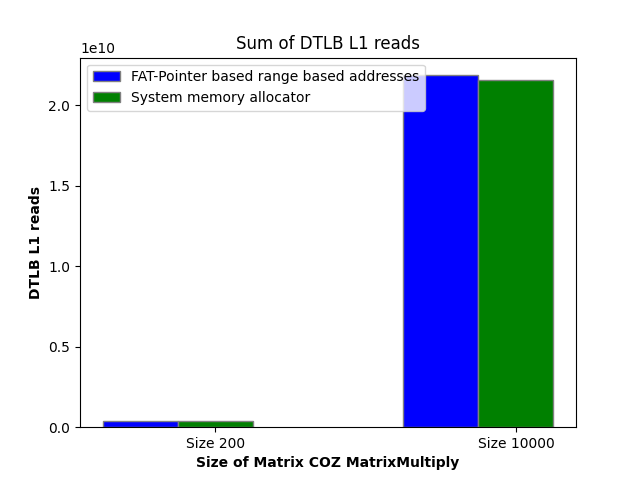
\includegraphics[width=.5\linewidth]{l1-tlb-matrixmultiply.png}\hfill
  \includegraphics[width=.5\linewidth]{l1-tlb-histogram.png}
  \caption{DTLB L1 reads}
\end{subfigure}
\end{figure}

\subsection{DTLB L2 reads:}
Similar to how L1 TLB reads are counted, DTLB L2 counts every read operation that accesses the 
Level 2 data or unified TLB. Each time there is a read to an entry in the Level 2 TLB, 
it is counted by the DTLB L2. 

% L2 TLB graphs
\begin{figure}
  \begin{subfigure}{\linewidth}
    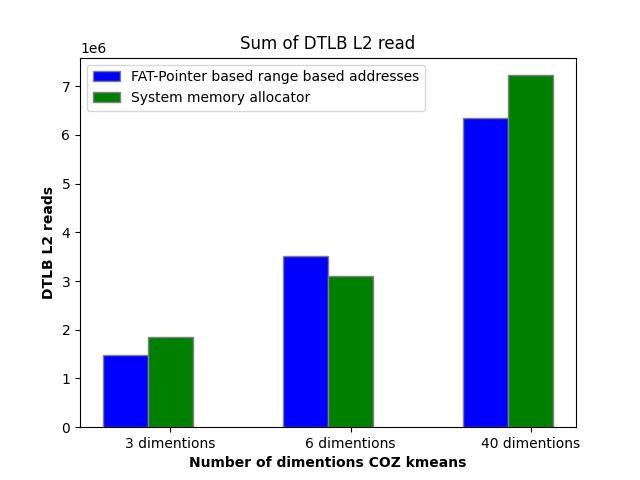
\includegraphics[width=.5\linewidth]{l2-tlb-kmeans.png}\hfill
    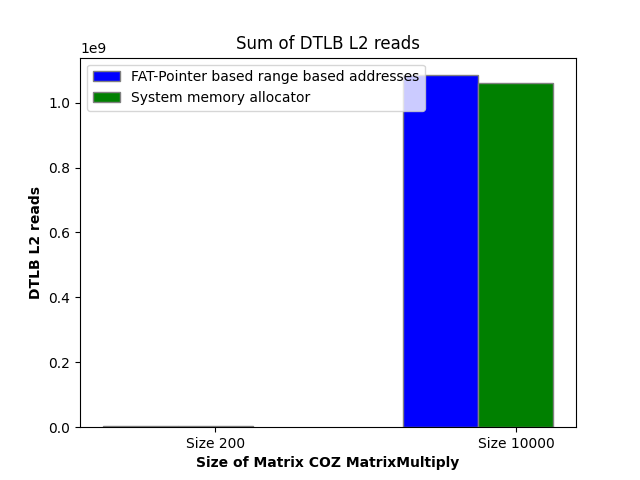
\includegraphics[width=.5\linewidth]{l2-tlb-matrixmultiply.png}\hfill
    \includegraphics[width=.5\linewidth]{l2-tlb-histogram.png}
  \caption{DTLB L2 reads}
\end{subfigure}
\end{figure}

% DTLB walks
% - Explain how the stat is calculated 
% - Fix older paragraphs 

\subsection{DTLB walks:}
The DTLB walk counter counts each Memory-read operation or Memory-write operation that causes a 
TLB access to at least the Level 2 data or unified TLB.
Each access to a TLB entry is counted including refills 
of Level 1 TLBs.

\begin{figure}
  \begin{subfigure}{\linewidth}
    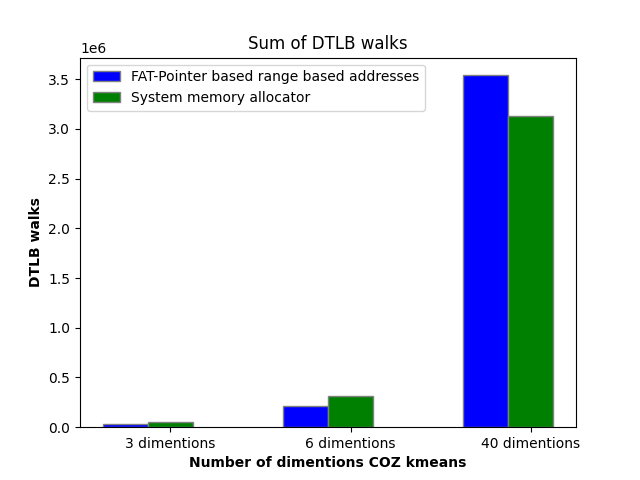
\includegraphics[width=.5\linewidth]{tlb-walk-kmeans.png}\hfill
    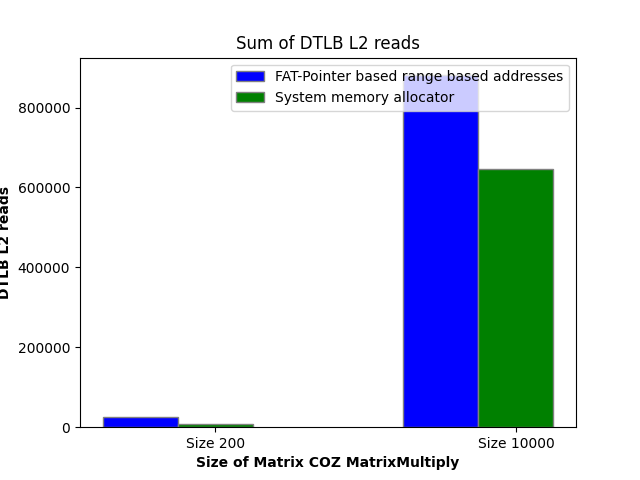
\includegraphics[width=.5\linewidth]{tlb-walk-matrixmultiply.png}\hfill
    \includegraphics[width=.5\linewidth]{tlb-walk-histogram.png}
  \caption{DTLB Walks}
\end{subfigure}
\end{figure}

% L1 cache miss
\subsection{L1 cache miss:}
L1 cache miss counter counts each Memory-read operation to the Level 1 data or unified cache counted by L1 cache miss counter that incurs additional latency because it returns data from outside of the Level 1 data or unified cache of this PE.
The event indicates to software that the access missed in the Level 1 data or unified cache and might have a significant performance impact due to the additional latency compared to the latency of an access that hits in the Level 1 data or unified cache.
% • Accesses where the additional latency is unlikely to be significantly performance-impacting. For example, if the access hits in another cache in the same local cluster, and the additional latency is small when compared to a miss in all Level 1 caches that the access looks up in and results in an access being made to a Level 2 cache or elsewhere beyond the Level 1 data or unified cache.
% • A miss that does not cause a new cache refill but is satisfied from a previous miss.

\begin{figure}
  \begin{subfigure}{\linewidth}
    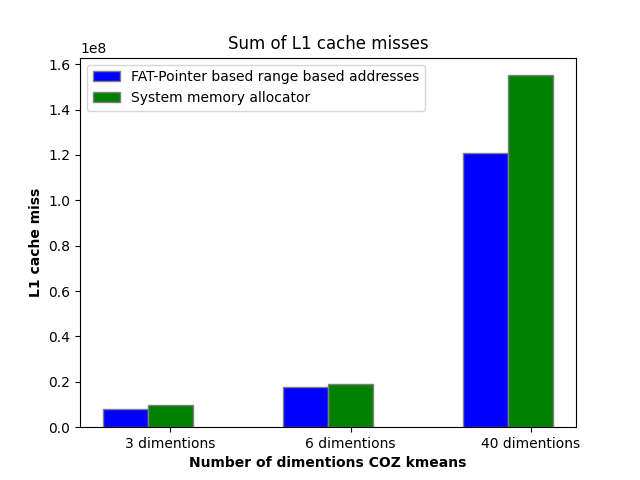
\includegraphics[width=.5\linewidth]{l1-miss-kmeans.png}\hfill
    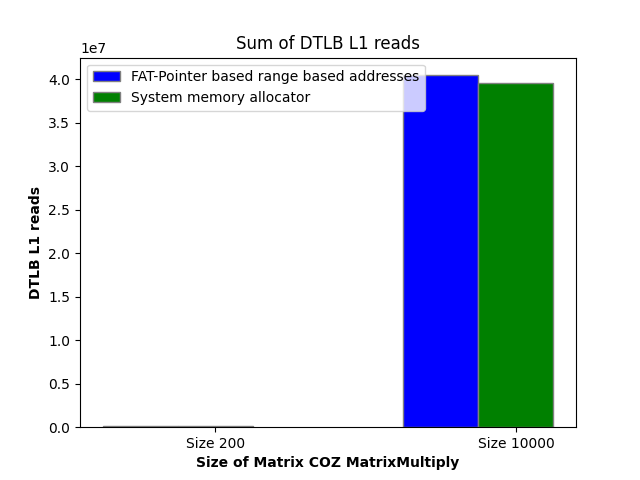
\includegraphics[width=.5\linewidth]{l1-miss-matrixmultiply.png}\hfill
    \includegraphics[width=.5\linewidth]{l1-miss-histogram.png}
  \caption{Cache misses}
\end{subfigure}
\end{figure}